%
% This document is available under the Creative Commons Attribution-ShareAlike
% License; additional terms may apply. See
%   * http://creativecommons.org/licenses/by-sa/3.0/
%   * http://creativecommons.org/licenses/by-sa/3.0/legalcode
%
% Created: 2012-07-28 20:09:12+02:00
% Main authors:
%     - Jérôme Pouiller <jezz@sysmic.org>
%

\part{Les systèmes de fichiers}

\begin{frame}
  \partpage
\end{frame}

\begin{frame}
  \tableofcontents[currentpart]
\end{frame}

\section{L'arborescence}

\begin{frame}[fragile=singleslide]{Généralités}
  Les types de fichiers
  \begin{itemize}
  \item Normal (\man{touch(1)}, \man{open(2)}, \man{mknod(2)})
  \item Répertoire (\man{mkdir(1)}, \man{mkdir(2)})
  \item Lien symbolique (\man{ln(1)}, \man{symblink(2)})
  \item Pipe nommé (\man{mkfifo(1)}, \man{mkfifo(3)}, \man{mknod(2)})
  \item Socket nommé (\man{bind(2)}, \man{mknod(2)})
  \item     Fichier    périphérique     charactère    (\man{mknod(1)},
    \man{mknod(2)})
  \item Fichier périphérique bloc (\man{mknod(1)}, \man{mknod(2)})
  \end{itemize}

  Par ailleurs, il  est possible de faire pointer  une nouvelle entrée
  vers une  structure de fichier existante.  Ce  mécanisme est appellé
  \emph{hard link}  (\man{ln(1)}, \man{link(2)}). Certain  système COW
  fonctionnes ainsi.
  \\
  Tous les caractères sont  autorisés sauf \c{/} (réservé pour séparer
  les  répertoires)  et \c{\\0}  (réservé  pour  indiquer  la fin  des
  arguments)
\end{frame}

\begin{frame}[fragile=singleslide]{Arborescence}
  Il s'agit  d'un standard, pour les systèmes  spécialisé, beaucoup de
  ces répertoire n'existeront pas.

  \man{debootstrap(1)} permet de crée une nouvelle arborescence et d'y
  décompresser   les   fichiers   minimum  au   fonctionnement   d'une
  distribution Debian

  Lorsque  vous  installez  (ou   compilez)  un  paquet,  vous  pouvez
  spécifier de l'installer à partir d'une autre racine.

  %   Peut-etre    à   mettre   dans   la   partie  virtualisation?
  Il  est possible  de s'exécuter  sur une  autre racine  à  l'aide de
  \man{chroot(1)}
\end{frame}

\begin{frame}[fragile=singleslide]{Arborescence}
  \begin{itemize}
  \item  \file{/bin}  \file{/sbin}  \file{/usr/bin}  \file{/usr/sbin}:
    Binaires
  \item \file{/} et \file{/usr} séparé pour des raison historiques
  \item \file{*/sbin}: Binaire normalement réservée à root
  \item \file{/lib*} \file{/usr/lib*}: Bibliothèque
  \item \file{/etc}:  Fichiers de configuration  système.  Beaucoup se
    terminent en \file{*rc.conf}
  \item \file{/home}, \file{/root} Espace des utilisateurs
  \end{itemize}
\end{frame}

\begin{frame}[fragile=singleslide]{Arborescence}
  \begin{itemize}
  \item \file{/var} Répertoire de travail des applications systèmes
  \item \file{/var/spool} Queue de traitement de certains démon (mail,
    imprimante, etc...)
  \item \file{/var/log} Logs système
  \item \file{/var/cache}  Cache système de certains  outils (index de
    man, version binaire des index apt, debconf, etc...)
  \item \file{/var/run} et  \file{/run} Fichier de communication entre
    les services  (fichiers de lock, PIDs,  sockets des communication,
    identifiants de mémoire partagée, etc...)
  \item  \file{/var/lib} Données de  travail de  certaine bibliothèque
    (apt, ...)
  \item \file{/var/www}, \file{/var/mail},  ...  Dédié aux partage web
    et mails
  \end{itemize}
\end{frame}

\begin{frame}[fragile=singleslide]{Arborescence}
  \begin{itemize}
  \item  \file{/usr/share}  Donnée   statiques  de  certains  services
    (icônes,  fonts,  internationalisation, configurations  statiques,
    etc...)
  \item \file{/usr/share/man} Pages de man
  \item \file{/usr/share/doc} Autre documentation, Licences
  \item  \file{/usr/include}  Fichiers  entêtes  des  bibliothèques  C
    (installés par les version \c{*-dev} des packets)
  \item \file{/usr/local} \file{/opt}  Application installée en dehors
    du service de packets normal (compilés localement)
  \item      \file{/tmp}       et      \file{/var/tmp}      Répertoire
    temporaire. \file{/tmp} est vidé à chaque redémarrage
  \end{itemize}
\end{frame}

\begin{frame}[fragile=singleslide]{Le répertoire \file{/dev}}
  \begin{itemize}
  \item Fichiers spéciaux, \emph{file devices}
  \item Communiquent avec des drivers (sous Unix, tout est fichier)
  \item \man{dd(1)}  permet un contrôle  plus fin et est  souvent plus
    approprié  que  \emph{cat}  et  \emph{echo}  pour  accéder  à  ces
    fichiers
  \item Certains  périphérique nécessite l'utilisation  d'autre appels
    système qui nous verrons plus tard
  \item Dans  tous les cas,  ces appels systèmes passent  utilisent un
    file descriptor comme identifiant
  \end{itemize}
\end{frame}

\begin{frame}[fragile=singleslide]{Le répertoire \file{/dev}}
  Quelques exemples:
  \begin{itemize}
  \item \file{/dev/ttyS0}: Premier port série
  \item \file{/dev/sda}: Premier disque
  \item \file{/dev/sr0}: Lecteur CD
  \item \file{/dev/mem}: Mémoire physique
  \item \file{/dev/zero}: Périphérique virtuel qui ne donne que des 0
  \item \file{/dev/random}: Source d'entropie
  \item \file{/dev/null}: Trou noir
  \item   \file{/dev/psaux}   et  \file{/dev/input/*}:   Périphériques
    d'entrées (souris, clavier, touchsreen, etc...)
  \item \file{/dev/snd/}: Cartes son
  \item \file{/dev/rtc0}: Horloge (plus spécial à accéder)
  \item \file{/dev/video0}, \file{/dev/nvidia}: Webcam, carte vidéo ne
    s'accèdent pas directement (nous y reviendrons)
  \end{itemize}
\end{frame}

\begin{frame}[fragile=singleslide]{Le répertoire \file{/dev}}
  N'apparaissent pas:
  \begin{itemize}
  \item Les bus (cas très rare et anormaux ou on fait des implémentations
    en userland),
  \item Les cartes  et les périphériques réseaux (à  l'heure du cloud et
    des environnement distribué, ca peut avoir son importance)
  \item  Les cartes  vidéo n'apparaissent  pas toujours.  Certains driver
    sont implémentés en userspace
  \end{itemize}
\end{frame}


\subsection{Les filesystems}

\begin{frame}[fragile=singleslide]{Les filesystems}
  \begin{itemize}
  \item Une  partition de disque est \emph{montée}  sur un \emph{point
      de montage}
  \item Un point de montage est un répertoire (vide de préférence)
  \item \man{mount(1)} \man{mount(2)} \man{mount(8)}
  \item  Il  existe  différent  type  de file  systemes:  vfat,  ntfs,
    iso9660, ext2, ext3, ext4, xfs, btrfs, reiserfs, cramfs, squashfs,
    jffs2
  \item  Il est  possible de  monter  un fichier  normal plutôt  qu'un
    fichier périphérique  avec \cmd{-o loop} (une image  disque ou une
    iso par exemple)
  \item \c{tmpfs} est mappé de sur de la mémoire RAM
  \item \c{procfs}  (monté sur  \file{/proc}) et \c{sysfs}  (monté sur
    \file{/sys}) sont des file systems virtuels
  \item Il permettent d'obtenir des informations sur l'état du noyau.
  \item Filesystems réseau: nfs, samba
  \item Filesystems plus complexes, implémenté en userland par FUSE (à
    l'aide de \file{/dev/fuse}): sshfs, ftpfs, etc..
  \end{itemize}
\end{frame}

\section{Implémentations}

\begin{frame}[fragile=singleslide]{Table des partitions}
  \begin{columns}
    \begin{column}{8cm}
      \begin{itemize}
      \item Inventée par Microsoft à peu près en même temps que la FAT
      \item CHS (Cylindre-Head-Sector) est  obsolete, de nos jours, on
        accède  au  disque  en   utilisant  leur  LBA  (Logical  Block
        Addressing)   (les  disque   IDE  doivent   implémenter  cette
        compatibilité, je ne crois pas que ca soit encore présent dans
        le protocole sata )
      \item Les 512 premiers octets représente la table
      \item Les 446 premiers octets contiennent le \emph{Bootcode} (un
        boot  loader s'appuyant  sur  le bios  encore  utilisé de  nos
        jours)
      \item Ensuite un tableau de  4 entré de 16 octets représentation
        4 partitions principales
      \item Chaque  entré contient le type, l'adresse  (LBA) de départ
        et la taille de la partition (répété dans le filesystem)
      \end{itemize}
    \end{column}
    \begin{column}{4cm}
      \includegraphics[height=5cm]{pics/mbr}
    \end{column}
  \end{columns}
\end{frame}

\subsection{VFAT}

\begin{frame}[fragile=singleslide]{Vfat}
  \begin{columns}
    \begin{column}{7cm}
  \begin{itemize}
  \item Acronyme de File Allocation Table
  \item Inventé par Microsoft en 1977
  \item Disque divisé en cluster de  $512 * 2^n$ octets (en fait $2^n$
    \emph{secteurs} de 512 octets)
  \item  La structure  volume ID  est  placée à  l'adresse zéro,  elle
    contient la taille des  cluster, l'adresse du répertoire racine et
    la taille de la FAT (nous  verrons que la taille de la partition =
    taille de fat en double mots * taille du cluster en octets)
  \end{itemize}
    \end{column}
    \begin{column}{5cm}
      \includegraphics[height=5cm]{pics/volume_id}
    \end{column}
  \end{columns}
\end{frame}

\begin{frame}[fragile=singleslide]{Les répertoires}
  Les répertoires
  \begin{itemize}
  \item Un  cluster répertoire est  un vecteur de  structures pointant
    sur des fichiers ou d'autres répertoire.
  \item Les entrée  contiennent un plus des information  comme le nom,
    la taille et les attribut des fichiers
    \begin{center}
      \includegraphics[height=0.8cm]{pics/dir_entry_short}
    \end{center}
  \item  Il existe  des valeurs  spéciales pour  indiquer  les entrées
    supprimées et la fin du listing
  \item On peut ainsi parcourir les fichier du disque
  \end{itemize}
\end{frame}

\begin{frame}[fragile=singleslide]{La FAT}
  Et si le fichier ou le répertoire ne tient pas sur un cluster?
  \begin{columns}
    \begin{column}{7cm}
      \begin{itemize}
      \item La FAT intervient
      \item La FAT est un tableau de d'entiers de 32bits (ou 16bits ou
        12 bits)
      \item Chaque  entrée représente un cluster (entrée  1 == cluster
        1)
      \item  Si  l'entrée  vaut  0,  le cluster  est  disponible  pour
        l'allocation
      \item Si  l'entrée vaut un nombre,  le cluster est  occupé et la
        valeur de l'entrée pointe sur le cluster suivant
      \item Si l'entrée vaut  \c{0xFFFFFFFF}, le cluster est occupé et
        c'est le dernier cluster du fichier ou du répertoire
      \end{itemize}
    \end{column}
    \begin{column}{5cm}
      \includegraphics[height=4cm]{pics/fat_sector}
    \end{column}
  \end{columns}
\end{frame}

\begin{frame}[fragile=singleslide]{La FAT}
  Les défauts:
  \begin{itemize}
  \item  La fragmentation  des données,  particulièrement vraie  si un
    fichier grossi progressivement
  \item Le  temps d'accès entre la  FAT et les données  et l'entrée du
    répertoire (pour modifier la taille)
  \item Le temps  d'accès entre la taille du  fichier (stockée avec le
    répertoire) et les données
  \item  La liste  simplement  chaînée dans  la  FAT qui  oblige à  la
    parcourir pour accéder à la fin du fichier
  \item Pas de pointeur vers le répertoire parent
  \end{itemize}
  cf. \url{http://www.pjrc.com/tech/8051/ide/fat32.html}
\end{frame}

\subsection{Ext2}

\begin{frame}[fragile=singleslide]{L'Ext2}
  \begin{itemize}
  \item Inventé par Rémy Card au LIP6
  \item Deux type de structures principales:
    \begin{itemize}
    \item Des inodes (index-node) (128bits)
    \item Des blocks (paramètrable de l'ordre de 4Ko de nos jours)
    \end{itemize}
  \item Les disque  est divisé en \emph{block group}  (une centaine de
    Mo)
  \item Le système de block group permet de rapprocher les données des
    index
  \item  ... et  de  plus facilement  récupérer  le disque  en cas  de
    problème
  \item Le premier  block groupe se trouve à  l'adresse 1024 (l'espace
    avant est réservé pour un éventuel bootloader)
  \end{itemize}
\end{frame}

\begin{frame}[fragile=singleslide]{Les block groups}
  Chaque \emph{block group} contient
  \begin{itemize}
  \item Une copie du  superblock (sauf si l'opton \emph{sparse\_block}
    est active)
  \item Des  données concernant ce  block (taille de  l'espace d'inode,
    taille  de  l'espace de  block,  nombre  de block/inode  utilisée,
    etc...)
  \item Un espace (fixe) d'inode
  \item Un espace (fixe) de block
  \item Un  pointeur vers un block  de bitmap des inode  qui permet de
    connaître les inodes alloués
  \item Une pointeur  vers un block de bitmap des  block qui permet de
    connaître les blocks alloués
  \end{itemize}
  \begin{center}
    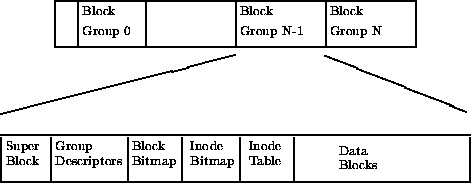
\includegraphics[height=2.5cm]{pics/img82}
  \end{center}
\end{frame}

\begin{frame}[fragile=singleslide]{Les block groups}
  \begin{itemize}
  \item  Remarque: Le bitmap  de block  doit tenir  sur un  block, par
    conséquent, il  ne peut y avoir  plus de (block\_size  * 8) blocks
    par  block group.  (aussi vrai  dans une  moindre mesure  pour les
    inodes).  C'est généralement ca  qui va déterminier la taille d'un
    groupe.
  \item  Remarque: En  connaissant,  la taille  des  block groups,  le
    nombre d'inode  par block  group et l'offset  de la  table d'inode
    dans  un group,  il est  possible d'indexer  n'importe  quel inode
    (idem pour les blocks)
  \end{itemize}
\end{frame}

\begin{frame}[fragile=singleslide]{Les inodes}
  Chaque fichier est associé à un inode. Un inode contient:
  \begin{itemize}
  \item Des  informations comme la  taille, les date  de modification,
    des création et d'accès, le type, etc...
  \item  Dans le  cas fichier  spéciaux, toutes  les  information sont
    contenus dans l'inode
  \item Un tableau  de 12 pointeur vers les  blocks contenant le corps
    du fichier (permet d'indexer les 50 premiers Ko)
  \item  Un pointeur  vers un  block contenant  des pointeurs  vers le
    corps du fichier (permet d'indexer les 4Mo suivants)
  \item un pointeur  vers un block de second  niveau (qui contient des
    pointeurs de pointeurs) (permet d'indexer les 4Go suivants)
  \item  un  pointeur vers  un  block  de  troisième niveau  (les  4To
    suivants)
    % \item  Le jours  ou ont aura  besoin d'indexer des  fichier de
    %   4Po, on ajoutera  une inférence (limite théorique de l'ordre
    %   de 10^40)
  \item Plus  le fichier est  gros, plus le nombre  d'indirections sera
    important
  \item Le système alloue en  priorité les fichiers dans le même block
    group que son inode (limite la fragmentation)
  \end{itemize}
\end{frame}

\begin{frame}[fragile=singleslide]{Les inodes}
  \begin{center}
    \includegraphics[height=6cm]{pics/Ext2-inode}
  \end{center}
  Remarque: les  premières inodes  du disque sont  réservée pour  : la
  liste des badblocks, le répertoire racine, le journal, etc...
\end{frame}

\begin{frame}[fragile=singleslide]{Les répertoires}
  \begin{columns}
    \begin{column}{4.5cm}
      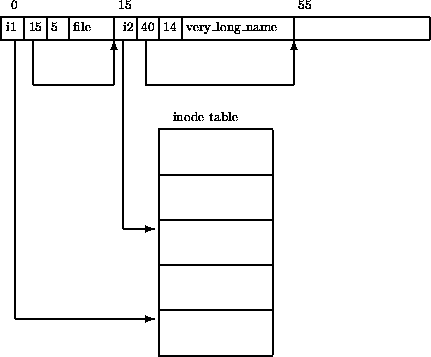
\includegraphics[height=6cm]{pics/img88}
    \end{column}
    \begin{column}{6.5cm}
      \\[3em]
      Un fichier peut-être un répertoire
      \begin{itemize}
      \item Il contient un  tableau de structures contenant l'inode du
        fichier, la taille du nom et le nom de l'entrée
      \item Un  répertoire contient systématiquement  une entrée \c{.}
        et une entrée \c{..}
      \item Une entrée dont l'inode est a zero à été supprimée
      \item Le parcours  des réperoitre se fait en  $O(n)$, un index à
        été ajouté sur ext3 pour le faire en $O(log_2(n))$
      \end{itemize}
    \end{column}
  \end{columns}

  cf.   \man{tune2fs(1)},  \man{debugfs(1)},  \man{stat(1)},
    \url{http://www.nongnu.org/ext2-doc/ext2.html}
  % Presnter le fonctionnement de fsck.ext2 (c'est interressant)
  % Exo: cacher des fichier dans de l'ext2 (il faut trouver de l'espace, ecrire, et activer la bitmap)
\end{frame}

\subsection{La journalisation}

\begin{frame}[fragile=singleslide]{Journalisation}
  \begin{itemize}
  \item Provient des technologies des bases de données
  \item Permet de garantir l'atomicité des opérations sur le disque
  \item On  écrit d'abord  dans le  journal ce que  l'on se  prépare à
    faire
  \item  Une fois  l'action écrite,  on  écrit ensuite  un message  de
    \emph{commit}
  \item Si le système plante, il  lit le journal, si une opération est
    associée à un commit, il exécute l'opération, sinon, on estime que
    les information  concernant l'opération sont  peut-être erronée et
    on exécute pas l'action
  \end{itemize}
\end{frame}

\begin{frame}[fragile=singleslide]{Journalisation}
  Evidement, il faut  de temps en temps écrire  réellement les données
  sur le disque.
  \begin{itemize}
  \item On commence par écrire les données
  \item On s'assure qu'elle ont été correctement écrite
  \item  Même si  le système  plante à  ce moment,  on  pourra rejouer
    l'entrée du journal
  \item on supprime l'entrée du journal
  \item Pour des raisons de performance, les entrée du journal ne sont
    pas forcement  écrite dans l'ordre. Il faut  alors faire attention
    aux contrainte de précédences
  \end{itemize}
  \begin{lstlisting}
$ debugfs -R logdump /dev/sda8
  \end{lstlisting}
\end{frame}

\begin{frame}[fragile=singleslide]{Journalisation}
  \begin{itemize}
  \item Il  est possible de  journaliser toutes les données  écrite ou
    seulement les meta donnée
  \item Dans le  second cas, on garanti que  filesystème sera cohérent
    mais pas les donnée à l'intérieur du fichier
  \item Linux implémente aussi  un mode \emph{ordered} qui garanti que
    les donnée sont  mise à jour sur le disque avant  de mettre à jour
    les meta  donnée. Ainsi,  il est possible  de perdre  des données,
    mais pas d'avoir des donnée corrompues.
  \end{itemize}
\end{frame}

\begin{frame}[fragile=singleslide]{Copy On Write}
  \begin{itemize}
  \item Certain file système sont dit Copy-On-Write
  \item Il sont montés read-only
  \item Si  un fichier dit  être modifié, une  copie est faite  (sur un
    autre espace ou en mémoire) et la copie est modifiée.
  \item Les futur accès ce feront sur la copie
  \item Permet de faire démarrer des  systèmes sur CD (avec un plus une
    compression dans ce cas)
  \item Permet  de faire fonctionner plusieurs système  sur une unique
    partition montée en lecture seule (virtualisation)
  \item Permet de démarrer des  machine en réseau avec un unique disque
    partagé
  \end{itemize}
\end{frame}

\section{Les RAID}

\begin{frame}[fragile=singleslide]{RAID}
  \begin{itemize}
  \item \emph{Redundant Array of Independent Disks}
  \item Peut-être matériel et transparent pour l'OS
  \item Software (cf. \man{mdadm(8)}). Le CPU doit alors s'occuper des
    différents calcul
  \item Apporte:
    \begin{itemize}
    \item Sécurité (Redondance)
    \item Performance
    \item Souplesse
    \end{itemize}
  \item  Données  regroupées en  bandes  (\emph{stripes}) de  quelques
    dizaines de kilo octets
  \item  Une  grappe  RAID est  vu  comme  un  unique disque  par  les
    filesystems de couches supérieur
  \end{itemize}
\end{frame}


\begin{frame}[fragile=singleslide]{RAID 0}
  \begin{columns}
    \begin{column}{6cm}
      \begin{itemize}
      \item Appelé \emph{Agrégation}
      \item Pas de redondance
      \item La capacité  totale est égale à la  somme des capacité des
        disques
      \item Permet de diviser les temps de lecture et écriture par $n$
      \end{itemize}
    \end{column}
    \begin{column}{4cm}
      \includegraphics[height=7cm]{pics/RAID_0}
    \end{column}
  \end{columns}
\end{frame}

\begin{frame}[fragile=singleslide]{RAID 1}
  \begin{columns}
    \begin{column}{6cm}
      \begin{itemize}
      \item Redondé $n$ fois. Permet d'avoir $n-1$ disques défaillants
      \item  La capacité  totale est  égale  la taille  du plus  petit
        disque de la grappe
      \item Pas de gain en  écriture, mais permet de diviser les temps
        d'écriture par $n$
      \end{itemize}
    \end{column}
    \begin{column}{4cm}
      \includegraphics[height=7cm]{pics/RAID_1}
    \end{column}
  \end{columns}
\end{frame}

\begin{frame}[fragile=singleslide]{RAID 2 et 3}
  \begin{itemize}
  \item Peu utilisé
  \item RAID 2: RAID 0 + ECC sur un disque séparé
  \item RAID 3: RAID 0 +  parité XOR  sur un disque séparé
    \includegraphics[height=5cm]{pics/RAID_2}
  \end{itemize}
\end{frame}

\begin{frame}[fragile=singleslide]{RAID 2 et 3}
  \begin{itemize}
  \item La parité se fait au niveau de l'octet.
  \item Les disque doivent être synchrone dans leur déplacement
  \item Les performances sont limités par le disque le plus lent
  \item Permettait de garantir la validité des données lues
  \item  ... mais,  un disque  est déjà  capable de  garantir  que les
    données sont correctes
  \item ... lors  des accès en lecture, on utilise  aussi le disque de
    parité alors que ca n'est pas utile
  \item Manque de flexibilité
  \end{itemize}
\end{frame}

\begin{frame}[fragile=singleslide]{RAID 3}
  \begin{lstlisting}
Drive #1: 00101010 (Data)
Drive #2: 10001110 (Data)
Drive #3: 11110111 (Data)
Drive #4: 10110101 (Data)
Drive #5: -------- (Hot Spare)
Drive #6: 11100110 (Parity)
  \end{lstlisting}
\end{frame}

\begin{frame}[fragile=singleslide]{RAID 3}
  \begin{lstlisting}
Drive #1: 00101010 (Data)
Drive #2:   dead   (Data)
Drive #3: 11110111 (Data)
Drive #4: 10110101 (Data)
Drive #5: -------- (Hot Spare)
Drive #6: 11100110 (Parity)
\end{lstlisting}
\end{frame}

\begin{frame}[fragile=singleslide]{RAID 3}
  \begin{lstlisting}
Drive #1: 00101010 (Data)
Drive #2:   dead   (Data)
Drive #3: 11110111 (Data)
Drive #4: 10110101 (Data)
Drive #5: 10001110 (Hot Spare)
Drive #6: 11100110 (Parity)
\end{lstlisting}
\end{frame}

\begin{frame}[fragile=singleslide]{RAID 4}
  \begin{itemize}
  \item RAID 0 + parité XOR  sur un disque séparé
  \item Ressemble au RAID 3
  \item Fonctionne par bloc plutôt que par octet
  \item Chaque disque fonctionne de manière asynchrone
  \item Permet d'optimiser les accès lecture/écriture
  \item Disymétrie  de l'usage  des disques: le  disque de  parité est
    sollicité à chaque écriture  (exemple: écritures sur les blocs A1,
    B2 et C3)
  \end{itemize}
  \begin{center}
    \includegraphics[height=4cm]{pics/RAID_4}
  \end{center}
\end{frame}

\begin{frame}[fragile=singleslide]{RAID 5}
  \begin{itemize}
  \item Evolution du RAID 4
  \item Le disque de parité n'est pas fixé
  \item Permet d'uniformiser l'usage des disques
  \end{itemize}
  \begin{center}
    \includegraphics[height=6cm]{pics/RAID_5}
  \end{center}
\end{frame}

\begin{frame}[fragile=singleslide]{RAID 6}
  \begin{itemize}
  \item Il arrive que l'opérateur change le mauvais disque
  \item  ...  ou  qu'un  second  disque  tombe  en  panne  pendant  la
    reconstruction (la loi des séries)
  \item  Remarque: Multiplier  le nombre  de disque  de parité  sur un
    RAID5 ne fonctionne pas (imaginez le cas ou deux disque de données
    tombent)
  \item L'objectif de RAID 6 est de permettre la perte de deux disques
    (ou lieu d'un seul avec le RAID 5)
  \end{itemize}
  \begin{center}
    \includegraphics[height=4cm]{pics/RAID_6}
  \end{center}
\end{frame}

\begin{frame}[fragile=singleslide]{RAID 6}
  \begin{itemize}
  \item On  utilise des codes  correcteurs de Reed-Solomon au  lieu du
    simple XOR
  \item Il est théoriquement  possible d'avoir des RAID6 permettant un
    nombre arbitraire de disque fautifs
  \item Les  implémentations actuelle  sont optimisées pour  2 disques
    fautifs
  \item Concrètement,  dans le  cas le plus  courant, on  utilise deux
    algorithmes de parités indépendants
    \begin{itemize}
    \item Le premier est un XOR classique (parité P)
    \item Le second est un XOR en appliquant tout d'abord une rotation
      de $i$ bits sur chaque octet du disque $i$ (parité Q).
    \end{itemize}
  \item Le RAID6 demande beaucoup de CPU pour calculer la parité Q. Il
    est souvent utilisé en hardware
  \end{itemize}
\end{frame}

\begin{frame}[fragile=singleslide]{RAID 6}
  Ainsi (grosso-modo, la parité Q se calcule ``en diagonale''):
  \begin{lstlisting}
Drive #1: 00101010 (Data)
Drive #2: 10001110 (Data)
Drive #3: 11110111 (Data)
Drive #4: 10110101 (Data)
Drive #5: 11100110 (Parity P)
Drive #6: 00100110 (Parity Q)
  \end{lstlisting}
\end{frame}

\begin{frame}[fragile=singleslide]{Les associations}
  \begin{itemize}
  \item Principalement utilisé pour les RAID 0 et 1
  \item A coût égal, moins performant qu'un RAID 5 ou 6
  \item  Peut néanmoins être  préférable dans  certains environnements
    techniques.
  \end{itemize}
  \begin{center}
    \includegraphics[height=5cm]{pics/RAID_01}
    \includegraphics[height=5cm]{pics/RAID_10}
  \end{center}
\end{frame}

\subsection{Un cas concret}

\begin{frame}[fragile=singleslide]{Exemple}
  Création d'un disque virtuel \c{/dev/md0}, en RAID-5 avec 3 disques:
  \begin{lstlisting}
# mdadm --create --verbose /dev/md0 --level=5 --chunk=128ko --raid-devices=3 /dev/sda1 /dev/sdb1 /dev/sdc1
# mdadm --detail /dev/md0
/dev/md0:
[...]
 Number   Major   Minor   RaidDevice State
    0       8        1        0      active sync   /dev/sda1
    1       8       17        1      active sync   /dev/sdb1
    2       8       33        2      active sync   /dev/sdc1
  \end{lstlisting}
\end{frame}

\begin{frame}[fragile=singleslide]{Exemple}
  Après un redémarrage, il faut \emph{réassembler} le RAID:
  \begin{lstlisting}
# mdadm --assemble /dev/md0 /dev/sda1 /dev/sdb1 /dev/sdc1
  \end{lstlisting}
  ou  en scannant  les partitions  (chaque élément  du RAID  contient un
  superblock      contenant     un      identifiant      unique     de
  RAID. cf. \url{https://raid.wiki.kernel.org/index.php/RAID_superblock_formats}).
  \begin{lstlisting}
# mdadm --assemble --scan
  \end{lstlisting}
  Cette  opération  est  normalement  faite  automatiquement  par  les
  scripts de démarrage du système
\end{frame}

\begin{frame}[fragile=singleslide]{Exemple}
  Marquer un disque  défaillant (pour un test ou  parce que des erreur
  ont été détectées):
  \begin{lstlisting}
# mdadm --fail /dev/md0 /dev/sdb1
# mdadm --detail /dev/md0
/dev/md0:
[...]
Rebuild Status : 6% complete
[...]
 Number   Major   Minor   RaidDevice State
    0       8        1        0      active sync   /dev/sda1
    1       0        0        1      removed       -
    2       8       33        2      active sync   /dev/sdc1
    1       8       17        -      faulty spare  /dev/sdb1
  \end{lstlisting}
\end{frame}

\begin{frame}[fragile=singleslide]{Exemple}
  Ajout  d'un  nouveau  disque.   Le RAID  est  alors  automatiquement
  reconstruit:
  \begin{lstlisting}
# mdadm --add /dev/md0 /dev/sdd1
# mdadm --detail /dev/md0
/dev/md0:
[...]
Rebuild Status : 6% complete
[...]
 Number   Major   Minor   RaidDevice State
    0       8        1        0      active sync   /dev/sda1
    1       8       49        1      active sync   /dev/sdd1
    2       8       33        2      active sync   /dev/sdc1
    3       8       17        -      faulty spare  /dev/sdb1
  \end{lstlisting}
  Attendre la reconstruction:
  \begin{lstlisting}
# mdadm --wait /dev/md0
  \end{lstlisting}
\end{frame}

\begin{frame}[fragile=singleslide]{Exemple}
  Retirer le disque fautif:
  \begin{lstlisting}
# mdadm --remove /dev/md0 /dev/sdb1
# mdadm --detail /dev/md0
/dev/md0:
[...]
Rebuild Status : 6% complete
[...]
 Number   Major   Minor   RaidDevice State
    0       8        1        0      active sync   /dev/sda1
    1       8       49        1      active sync   /dev/sdd1
    2       8       33        2      active sync   /dev/sdc1
  \end{lstlisting}
\end{frame}

\begin{frame}[fragile=singleslide]{Exemple}
  Ajout d'un nouveau  disque de spare.  Ainsi, si  un nouveau disque a
  une défaillance,  il sera automatiquement remplacé par  le disque de
  spare:
  \begin{lstlisting}
# mdadm --add /dev/md0 /dev/sde1
# mdadm --detail /dev/md0
/dev/md0:
[...]
Rebuild Status : 6% complete
[...]
 Number   Major   Minor   RaidDevice State
    0       8        1        0      active sync   /dev/sda1
    1       8       49        1      active sync   /dev/sdd1
    2       8       33        2      active sync   /dev/sdc1
    3       8       65        -      spare         /dev/sde1
  \end{lstlisting}
\end{frame}

\begin{frame}[fragile=singleslide]{Exemple}
  Modifier le nombre de disque utilisés (pas forcement possible)
  \begin{lstlisting}
# mdadm --grow --raid-devices=4 /dev/md0
# mdadm --detail /dev/md0
/dev/md0:
[...]
Rebuild Status : 1% complete
[...]
 Number   Major   Minor   RaidDevice State
    0       8        1        0      active sync   /dev/sda1
    1       8       49        1      active sync   /dev/sdd1
    2       8       33        2      active sync   /dev/sdc1
    3       8       65        3      active sync   /dev/sde1
  \end{lstlisting}
\end{frame}
